%\documentclass{standalone}
%\usepackage{tikz}
%\usetikzlibrary{patterns,plotmarks}
%\begin{document}
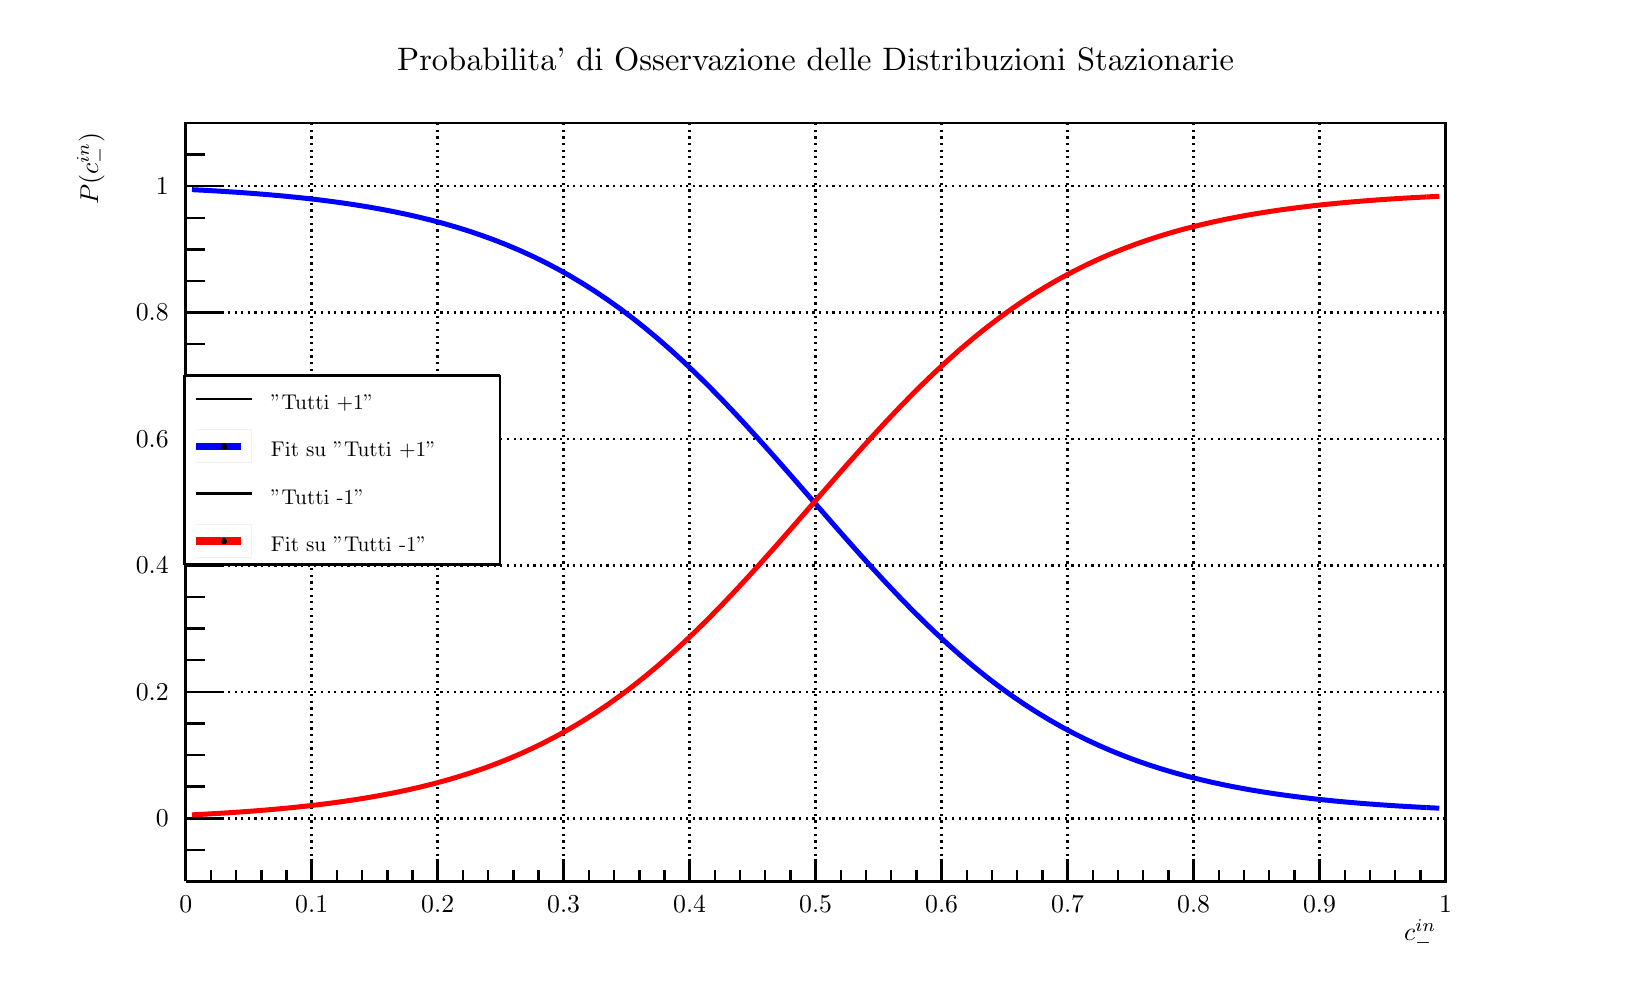
\begin{tikzpicture}
\def\CheckTikzLibraryLoaded#1{ \ifcsname tikz@library@#1@loaded\endcsname \else \PackageWarning{tikz}{usetikzlibrary{#1} is missing in the preamble.} \fi }
\CheckTikzLibraryLoaded{patterns}
\CheckTikzLibraryLoaded{plotmarks}
\pgfdeclareplotmark{cross} {
\pgfpathmoveto{\pgfpoint{-0.3\pgfplotmarksize}{\pgfplotmarksize}}
\pgfpathlineto{\pgfpoint{+0.3\pgfplotmarksize}{\pgfplotmarksize}}
\pgfpathlineto{\pgfpoint{+0.3\pgfplotmarksize}{0.3\pgfplotmarksize}}
\pgfpathlineto{\pgfpoint{+1\pgfplotmarksize}{0.3\pgfplotmarksize}}
\pgfpathlineto{\pgfpoint{+1\pgfplotmarksize}{-0.3\pgfplotmarksize}}
\pgfpathlineto{\pgfpoint{+0.3\pgfplotmarksize}{-0.3\pgfplotmarksize}}
\pgfpathlineto{\pgfpoint{+0.3\pgfplotmarksize}{-1.\pgfplotmarksize}}
\pgfpathlineto{\pgfpoint{-0.3\pgfplotmarksize}{-1.\pgfplotmarksize}}
\pgfpathlineto{\pgfpoint{-0.3\pgfplotmarksize}{-0.3\pgfplotmarksize}}
\pgfpathlineto{\pgfpoint{-1.\pgfplotmarksize}{-0.3\pgfplotmarksize}}
\pgfpathlineto{\pgfpoint{-1.\pgfplotmarksize}{0.3\pgfplotmarksize}}
\pgfpathlineto{\pgfpoint{-0.3\pgfplotmarksize}{0.3\pgfplotmarksize}}
\pgfpathclose
\pgfusepathqstroke
}
\pgfdeclareplotmark{cross*} {
\pgfpathmoveto{\pgfpoint{-0.3\pgfplotmarksize}{\pgfplotmarksize}}
\pgfpathlineto{\pgfpoint{+0.3\pgfplotmarksize}{\pgfplotmarksize}}
\pgfpathlineto{\pgfpoint{+0.3\pgfplotmarksize}{0.3\pgfplotmarksize}}
\pgfpathlineto{\pgfpoint{+1\pgfplotmarksize}{0.3\pgfplotmarksize}}
\pgfpathlineto{\pgfpoint{+1\pgfplotmarksize}{-0.3\pgfplotmarksize}}
\pgfpathlineto{\pgfpoint{+0.3\pgfplotmarksize}{-0.3\pgfplotmarksize}}
\pgfpathlineto{\pgfpoint{+0.3\pgfplotmarksize}{-1.\pgfplotmarksize}}
\pgfpathlineto{\pgfpoint{-0.3\pgfplotmarksize}{-1.\pgfplotmarksize}}
\pgfpathlineto{\pgfpoint{-0.3\pgfplotmarksize}{-0.3\pgfplotmarksize}}
\pgfpathlineto{\pgfpoint{-1.\pgfplotmarksize}{-0.3\pgfplotmarksize}}
\pgfpathlineto{\pgfpoint{-1.\pgfplotmarksize}{0.3\pgfplotmarksize}}
\pgfpathlineto{\pgfpoint{-0.3\pgfplotmarksize}{0.3\pgfplotmarksize}}
\pgfpathclose
\pgfusepathqfillstroke
}
\pgfdeclareplotmark{newstar} {
\pgfpathmoveto{\pgfqpoint{0pt}{\pgfplotmarksize}}
\pgfpathlineto{\pgfqpointpolar{44}{0.5\pgfplotmarksize}}
\pgfpathlineto{\pgfqpointpolar{18}{\pgfplotmarksize}}
\pgfpathlineto{\pgfqpointpolar{-20}{0.5\pgfplotmarksize}}
\pgfpathlineto{\pgfqpointpolar{-54}{\pgfplotmarksize}}
\pgfpathlineto{\pgfqpointpolar{-90}{0.5\pgfplotmarksize}}
\pgfpathlineto{\pgfqpointpolar{234}{\pgfplotmarksize}}
\pgfpathlineto{\pgfqpointpolar{198}{0.5\pgfplotmarksize}}
\pgfpathlineto{\pgfqpointpolar{162}{\pgfplotmarksize}}
\pgfpathlineto{\pgfqpointpolar{134}{0.5\pgfplotmarksize}}
\pgfpathclose
\pgfusepathqstroke
}
\pgfdeclareplotmark{newstar*} {
\pgfpathmoveto{\pgfqpoint{0pt}{\pgfplotmarksize}}
\pgfpathlineto{\pgfqpointpolar{44}{0.5\pgfplotmarksize}}
\pgfpathlineto{\pgfqpointpolar{18}{\pgfplotmarksize}}
\pgfpathlineto{\pgfqpointpolar{-20}{0.5\pgfplotmarksize}}
\pgfpathlineto{\pgfqpointpolar{-54}{\pgfplotmarksize}}
\pgfpathlineto{\pgfqpointpolar{-90}{0.5\pgfplotmarksize}}
\pgfpathlineto{\pgfqpointpolar{234}{\pgfplotmarksize}}
\pgfpathlineto{\pgfqpointpolar{198}{0.5\pgfplotmarksize}}
\pgfpathlineto{\pgfqpointpolar{162}{\pgfplotmarksize}}
\pgfpathlineto{\pgfqpointpolar{134}{0.5\pgfplotmarksize}}
\pgfpathclose
\pgfusepathqfillstroke
}
\definecolor{c}{rgb}{1,1,1};
\draw [color=c, fill=c] (0,0) rectangle (20,12.0401);
\draw [color=c, fill=c] (2,1.20401) rectangle (18,10.8361);
\definecolor{c}{rgb}{0,0,0};
\draw [c,line width=0.9] (2,1.20401) -- (2,10.8361) -- (18,10.8361) -- (18,1.20401) -- (2,1.20401);
\definecolor{c}{rgb}{1,1,1};
\draw [color=c, fill=c] (2,1.20401) rectangle (18,10.8361);
\definecolor{c}{rgb}{0,0,0};
\draw [c,line width=0.9] (2,1.20401) -- (2,10.8361) -- (18,10.8361) -- (18,1.20401) -- (2,1.20401);
\draw [c,line width=0.9] (2,1.20401) -- (18,1.20401);
\draw [c,dash pattern=on 0.80pt off 1.60pt ,line width=0.9] (2,10.8361) -- (2,1.20401);
\draw [c,dash pattern=on 0.80pt off 1.60pt ,line width=0.9] (3.6,10.8361) -- (3.6,1.20401);
\draw [c,dash pattern=on 0.80pt off 1.60pt ,line width=0.9] (5.2,10.8361) -- (5.2,1.20401);
\draw [c,dash pattern=on 0.80pt off 1.60pt ,line width=0.9] (6.8,10.8361) -- (6.8,1.20401);
\draw [c,dash pattern=on 0.80pt off 1.60pt ,line width=0.9] (8.4,10.8361) -- (8.4,1.20401);
\draw [c,dash pattern=on 0.80pt off 1.60pt ,line width=0.9] (10,10.8361) -- (10,1.20401);
\draw [c,dash pattern=on 0.80pt off 1.60pt ,line width=0.9] (11.6,10.8361) -- (11.6,1.20401);
\draw [c,dash pattern=on 0.80pt off 1.60pt ,line width=0.9] (13.2,10.8361) -- (13.2,1.20401);
\draw [c,dash pattern=on 0.80pt off 1.60pt ,line width=0.9] (14.8,10.8361) -- (14.8,1.20401);
\draw [c,dash pattern=on 0.80pt off 1.60pt ,line width=0.9] (16.4,10.8361) -- (16.4,1.20401);
\draw [c,dash pattern=on 0.80pt off 1.60pt ,line width=0.9] (18,10.8361) -- (18,1.20401);
\draw [c,line width=0.9] (2,1.20401) -- (2,10.8361);
\draw [c,dash pattern=on 0.80pt off 1.60pt ,line width=0.9] (18,2.00668) -- (2,2.00668);
\draw [c,dash pattern=on 0.80pt off 1.60pt ,line width=0.9] (18,3.61202) -- (2,3.61202);
\draw [c,dash pattern=on 0.80pt off 1.60pt ,line width=0.9] (18,5.21736) -- (2,5.21736);
\draw [c,dash pattern=on 0.80pt off 1.60pt ,line width=0.9] (18,6.82271) -- (2,6.82271);
\draw [c,dash pattern=on 0.80pt off 1.60pt ,line width=0.9] (18,8.42805) -- (2,8.42805);
\draw [c,dash pattern=on 0.80pt off 1.60pt ,line width=0.9] (18,10.0334) -- (2,10.0334);
\draw [c,dash pattern=on 0.80pt off 1.60pt ,line width=0.9] (18,2.00668) -- (2,2.00668);
\draw [c,dash pattern=on 0.80pt off 1.60pt ,line width=0.9] (18,10.0334) -- (2,10.0334);
\draw [c,line width=0.9] (2,1.20401) -- (18,1.20401);
\draw [c,line width=0.9] (2,1.49297) -- (2,1.20401);
\draw [c,line width=0.9] (2.32,1.34849) -- (2.32,1.20401);
\draw [c,line width=0.9] (2.64,1.34849) -- (2.64,1.20401);
\draw [c,line width=0.9] (2.96,1.34849) -- (2.96,1.20401);
\draw [c,line width=0.9] (3.28,1.34849) -- (3.28,1.20401);
\draw [c,line width=0.9] (3.6,1.49297) -- (3.6,1.20401);
\draw [c,line width=0.9] (3.92,1.34849) -- (3.92,1.20401);
\draw [c,line width=0.9] (4.24,1.34849) -- (4.24,1.20401);
\draw [c,line width=0.9] (4.56,1.34849) -- (4.56,1.20401);
\draw [c,line width=0.9] (4.88,1.34849) -- (4.88,1.20401);
\draw [c,line width=0.9] (5.2,1.49297) -- (5.2,1.20401);
\draw [c,line width=0.9] (5.52,1.34849) -- (5.52,1.20401);
\draw [c,line width=0.9] (5.84,1.34849) -- (5.84,1.20401);
\draw [c,line width=0.9] (6.16,1.34849) -- (6.16,1.20401);
\draw [c,line width=0.9] (6.48,1.34849) -- (6.48,1.20401);
\draw [c,line width=0.9] (6.8,1.49297) -- (6.8,1.20401);
\draw [c,line width=0.9] (7.12,1.34849) -- (7.12,1.20401);
\draw [c,line width=0.9] (7.44,1.34849) -- (7.44,1.20401);
\draw [c,line width=0.9] (7.76,1.34849) -- (7.76,1.20401);
\draw [c,line width=0.9] (8.08,1.34849) -- (8.08,1.20401);
\draw [c,line width=0.9] (8.4,1.49297) -- (8.4,1.20401);
\draw [c,line width=0.9] (8.72,1.34849) -- (8.72,1.20401);
\draw [c,line width=0.9] (9.04,1.34849) -- (9.04,1.20401);
\draw [c,line width=0.9] (9.36,1.34849) -- (9.36,1.20401);
\draw [c,line width=0.9] (9.68,1.34849) -- (9.68,1.20401);
\draw [c,line width=0.9] (10,1.49297) -- (10,1.20401);
\draw [c,line width=0.9] (10.32,1.34849) -- (10.32,1.20401);
\draw [c,line width=0.9] (10.64,1.34849) -- (10.64,1.20401);
\draw [c,line width=0.9] (10.96,1.34849) -- (10.96,1.20401);
\draw [c,line width=0.9] (11.28,1.34849) -- (11.28,1.20401);
\draw [c,line width=0.9] (11.6,1.49297) -- (11.6,1.20401);
\draw [c,line width=0.9] (11.92,1.34849) -- (11.92,1.20401);
\draw [c,line width=0.9] (12.24,1.34849) -- (12.24,1.20401);
\draw [c,line width=0.9] (12.56,1.34849) -- (12.56,1.20401);
\draw [c,line width=0.9] (12.88,1.34849) -- (12.88,1.20401);
\draw [c,line width=0.9] (13.2,1.49297) -- (13.2,1.20401);
\draw [c,line width=0.9] (13.52,1.34849) -- (13.52,1.20401);
\draw [c,line width=0.9] (13.84,1.34849) -- (13.84,1.20401);
\draw [c,line width=0.9] (14.16,1.34849) -- (14.16,1.20401);
\draw [c,line width=0.9] (14.48,1.34849) -- (14.48,1.20401);
\draw [c,line width=0.9] (14.8,1.49297) -- (14.8,1.20401);
\draw [c,line width=0.9] (15.12,1.34849) -- (15.12,1.20401);
\draw [c,line width=0.9] (15.44,1.34849) -- (15.44,1.20401);
\draw [c,line width=0.9] (15.76,1.34849) -- (15.76,1.20401);
\draw [c,line width=0.9] (16.08,1.34849) -- (16.08,1.20401);
\draw [c,line width=0.9] (16.4,1.49297) -- (16.4,1.20401);
\draw [c,line width=0.9] (16.72,1.34849) -- (16.72,1.20401);
\draw [c,line width=0.9] (17.04,1.34849) -- (17.04,1.20401);
\draw [c,line width=0.9] (17.36,1.34849) -- (17.36,1.20401);
\draw [c,line width=0.9] (17.68,1.34849) -- (17.68,1.20401);
\draw [c,line width=0.9] (18,1.49297) -- (18,1.20401);
\draw [anchor=base] (2,0.806685) node[scale=0.930461, color=c, rotate=0]{0};
\draw [anchor=base] (3.6,0.806685) node[scale=0.930461, color=c, rotate=0]{0.1};
\draw [anchor=base] (5.2,0.806685) node[scale=0.930461, color=c, rotate=0]{0.2};
\draw [anchor=base] (6.8,0.806685) node[scale=0.930461, color=c, rotate=0]{0.3};
\draw [anchor=base] (8.4,0.806685) node[scale=0.930461, color=c, rotate=0]{0.4};
\draw [anchor=base] (10,0.806685) node[scale=0.930461, color=c, rotate=0]{0.5};
\draw [anchor=base] (11.6,0.806685) node[scale=0.930461, color=c, rotate=0]{0.6};
\draw [anchor=base] (13.2,0.806685) node[scale=0.930461, color=c, rotate=0]{0.7};
\draw [anchor=base] (14.8,0.806685) node[scale=0.930461, color=c, rotate=0]{0.8};
\draw [anchor=base] (16.4,0.806685) node[scale=0.930461, color=c, rotate=0]{0.9};
\draw [anchor=base] (18,0.806685) node[scale=0.930461, color=c, rotate=0]{1};
\draw [anchor= east] (18,0.529763) node[scale=0.930461, color=c, rotate=0]{$ c^{in}_{-}$};
\draw [c,line width=0.9] (2,1.20401) -- (2,10.8361);
\draw [c,line width=0.9] (2.48,2.00668) -- (2,2.00668);
\draw [c,line width=0.9] (2.24,2.40801) -- (2,2.40801);
\draw [c,line width=0.9] (2.24,2.80935) -- (2,2.80935);
\draw [c,line width=0.9] (2.24,3.21069) -- (2,3.21069);
\draw [c,line width=0.9] (2.48,3.61202) -- (2,3.61202);
\draw [c,line width=0.9] (2.24,4.01336) -- (2,4.01336);
\draw [c,line width=0.9] (2.24,4.41469) -- (2,4.41469);
\draw [c,line width=0.9] (2.24,4.81603) -- (2,4.81603);
\draw [c,line width=0.9] (2.48,5.21736) -- (2,5.21736);
\draw [c,line width=0.9] (2.24,5.6187) -- (2,5.6187);
\draw [c,line width=0.9] (2.24,6.02004) -- (2,6.02004);
\draw [c,line width=0.9] (2.24,6.42137) -- (2,6.42137);
\draw [c,line width=0.9] (2.48,6.82271) -- (2,6.82271);
\draw [c,line width=0.9] (2.24,7.22404) -- (2,7.22404);
\draw [c,line width=0.9] (2.24,7.62538) -- (2,7.62538);
\draw [c,line width=0.9] (2.24,8.02672) -- (2,8.02672);
\draw [c,line width=0.9] (2.48,8.42805) -- (2,8.42805);
\draw [c,line width=0.9] (2.24,8.82939) -- (2,8.82939);
\draw [c,line width=0.9] (2.24,9.23072) -- (2,9.23072);
\draw [c,line width=0.9] (2.24,9.63206) -- (2,9.63206);
\draw [c,line width=0.9] (2.48,10.0334) -- (2,10.0334);
\draw [c,line width=0.9] (2.48,2.00668) -- (2,2.00668);
\draw [c,line width=0.9] (2.24,1.60534) -- (2,1.60534);
\draw [c,line width=0.9] (2.48,10.0334) -- (2,10.0334);
\draw [c,line width=0.9] (2.24,10.4347) -- (2,10.4347);
\draw [anchor= east] (1.9,2.00668) node[scale=0.930461, color=c, rotate=0]{0};
\draw [anchor= east] (1.9,3.61202) node[scale=0.930461, color=c, rotate=0]{0.2};
\draw [anchor= east] (1.9,5.21736) node[scale=0.930461, color=c, rotate=0]{0.4};
\draw [anchor= east] (1.9,6.82271) node[scale=0.930461, color=c, rotate=0]{0.6};
\draw [anchor= east] (1.9,8.42805) node[scale=0.930461, color=c, rotate=0]{0.8};
\draw [anchor= east] (1.9,10.0334) node[scale=0.930461, color=c, rotate=0]{1};
\draw [anchor= east] (0.808197,10.8361) node[scale=0.930461, color=c, rotate=90]{$ P (c^{in}_{-})$};
\definecolor{c}{rgb}{0,0,0.8};
\foreach \P in {(3.6,9.87286), (6.8,8.98992), (10,5.93977), (13.2,3.21069), (16.4,2.16721)}{\draw[mark options={color=c,fill=c},mark size=2.402402pt, line width=0.000000pt, mark=] plot coordinates {\P};}
\definecolor{c}{rgb}{0,0,1};
\draw [c,line width=1.8] (2.08,9.98983) -- (2.24,9.98153) -- (2.4,9.97244) -- (2.56,9.96251) -- (2.72,9.95165) -- (2.88,9.93978) -- (3.04,9.92681) -- (3.2,9.91265) -- (3.36,9.89718) -- (3.52,9.8803) -- (3.68,9.86188) -- (3.84,9.84179) -- (4,9.81988)
 -- (4.16,9.79601) -- (4.32,9.77002) -- (4.48,9.74173) -- (4.64,9.71096) -- (4.8,9.67752) -- (4.96,9.64119) -- (5.12,9.60178) -- (5.28,9.55904) -- (5.44,9.51275) -- (5.6,9.46266) -- (5.76,9.40853) -- (5.92,9.3501) -- (6.08,9.28711) -- (6.24,9.21931)
 -- (6.4,9.14645) -- (6.56,9.06826) -- (6.72,8.98452) -- (6.88,8.895) -- (7.04,8.7995) -- (7.2,8.69784) -- (7.36,8.58988) -- (7.52,8.4755) -- (7.68,8.35464) -- (7.84,8.2273) -- (8,8.0935) -- (8.16,7.95336) -- (8.32,7.80704) -- (8.48,7.65477) --
 (8.64,7.49687) -- (8.8,7.33373) -- (8.96,7.16578) -- (9.12,6.99355) -- (9.28,6.81763) -- (9.44,6.63867) -- (9.6,6.45733) -- (9.76,6.27437) -- (9.92,6.09053);
\draw [c,line width=1.8] (9.92,6.09053) -- (10.08,5.90658) -- (10.24,5.7233) -- (10.4,5.54144) -- (10.56,5.36174) -- (10.72,5.18491) -- (10.88,5.0116) -- (11.04,4.84241) -- (11.2,4.67788) -- (11.36,4.51848) -- (11.52,4.36461) -- (11.68,4.21661) --
 (11.84,4.07473) -- (12,3.93916) -- (12.16,3.81001) -- (12.32,3.68736) -- (12.48,3.57118) -- (12.64,3.46145) -- (12.8,3.35805) -- (12.96,3.26085) -- (13.12,3.16969) -- (13.28,3.08437) -- (13.44,3.00466) -- (13.6,2.93034) -- (13.76,2.86115) --
 (13.92,2.79686) -- (14.08,2.73719) -- (14.24,2.68189) -- (14.4,2.6307) -- (14.56,2.58338) -- (14.72,2.53968) -- (14.88,2.49936) -- (15.04,2.4622) -- (15.2,2.42798) -- (15.36,2.39648) -- (15.52,2.36752) -- (15.68,2.34091) -- (15.84,2.31647) --
 (16,2.29403) -- (16.16,2.27345) -- (16.32,2.25458) -- (16.48,2.23728) -- (16.64,2.22143) -- (16.8,2.20692) -- (16.96,2.19363) -- (17.12,2.18146) -- (17.28,2.17033) -- (17.44,2.16015) -- (17.6,2.15084) -- (17.76,2.14232);
\draw [c,line width=1.8] (17.76,2.14232) -- (17.92,2.13454);
\definecolor{c}{rgb}{0.8,0,0};
\foreach \P in {(3.6,2.16721), (6.8,3.05015), (10,6.1003), (13.2,8.82939), (16.4,9.87286)}{\draw[mark options={color=c,fill=c},mark size=2.402402pt, line width=0.000000pt, mark=] plot coordinates {\P};}
\definecolor{c}{rgb}{1,0,0};
\draw [c,line width=1.8] (2.08,2.05024) -- (2.24,2.05855) -- (2.4,2.06763) -- (2.56,2.07756) -- (2.72,2.08842) -- (2.88,2.10029) -- (3.04,2.11326) -- (3.2,2.12742) -- (3.36,2.14289) -- (3.52,2.15977) -- (3.68,2.17819) -- (3.84,2.19829) -- (4,2.22019)
 -- (4.16,2.24406) -- (4.32,2.27005) -- (4.48,2.29834) -- (4.64,2.32911) -- (4.8,2.36256) -- (4.96,2.39888) -- (5.12,2.4383) -- (5.28,2.48103) -- (5.44,2.52732) -- (5.6,2.57741) -- (5.76,2.63154) -- (5.92,2.68997) -- (6.08,2.75296) -- (6.24,2.82076)
 -- (6.4,2.89363) -- (6.56,2.97181) -- (6.72,3.05555) -- (6.88,3.14507) -- (7.04,3.24057) -- (7.2,3.34223) -- (7.36,3.4502) -- (7.52,3.56457) -- (7.68,3.68543) -- (7.84,3.81277) -- (8,3.94657) -- (8.16,4.08671) -- (8.32,4.23304) -- (8.48,4.3853) --
 (8.64,4.5432) -- (8.8,4.70635) -- (8.96,4.87429) -- (9.12,5.04652) -- (9.28,5.22244) -- (9.44,5.40141) -- (9.6,5.58274) -- (9.76,5.7657) -- (9.92,5.94954);
\draw [c,line width=1.8] (9.92,5.94954) -- (10.08,6.13349) -- (10.24,6.31677) -- (10.4,6.49863) -- (10.56,6.67833) -- (10.72,6.85516) -- (10.88,7.02847) -- (11.04,7.19766) -- (11.2,7.3622) -- (11.36,7.52159) -- (11.52,7.67546) -- (11.68,7.82346) --
 (11.84,7.96534) -- (12,8.10091) -- (12.16,8.23006) -- (12.32,8.35272) -- (12.48,8.46889) -- (12.64,8.57863) -- (12.8,8.68202) -- (12.96,8.77922) -- (13.12,8.87038) -- (13.28,8.95571) -- (13.44,9.03541) -- (13.6,9.10974) -- (13.76,9.17892) --
 (13.92,9.24322) -- (14.08,9.30289) -- (14.24,9.35819) -- (14.4,9.40937) -- (14.56,9.45669) -- (14.72,9.50039) -- (14.88,9.54071) -- (15.04,9.57787) -- (15.2,9.6121) -- (15.36,9.64359) -- (15.52,9.67255) -- (15.68,9.69916) -- (15.84,9.7236) --
 (16,9.74604) -- (16.16,9.76662) -- (16.32,9.78549) -- (16.48,9.80279) -- (16.64,9.81864) -- (16.8,9.83315) -- (16.96,9.84644) -- (17.12,9.85861) -- (17.28,9.86974) -- (17.44,9.87992) -- (17.6,9.88924) -- (17.76,9.89775);
\draw [c,line width=1.8] (17.76,9.89775) -- (17.92,9.90554);
\definecolor{c}{rgb}{1,1,1};
\draw [color=c, fill=c] (1.98543,5.22769) rectangle (5.99271,7.63206);
\definecolor{c}{rgb}{0,0,0};
\draw [c,line width=0.9] (1.98543,5.22769) -- (5.99271,5.22769);
\draw [c,line width=0.9] (5.99271,5.22769) -- (5.99271,7.63206);
\draw [c,line width=0.9] (5.99271,7.63206) -- (1.98543,7.63206);
\draw [c,line width=0.9] (1.98543,7.63206) -- (1.98543,5.22769);
\draw [anchor=base west] (2.98725,7.19627) node[scale=0.768642, color=c, rotate=0]{"Tutti +1"};
\definecolor{c}{rgb}{1,1,1};
\draw [c, fill=c] (2.1357,7.12113) -- (2.83698,7.12113) -- (2.83698,7.54189) -- (2.1357,7.54189);
\definecolor{c}{rgb}{0,0,0};
\draw [c,line width=0.9] (2.1357,7.33151) -- (2.83698,7.33151);
\definecolor{c}{rgb}{0,0,0.8};
\foreach \P in {(2.48634,7.33151)}{\draw[mark options={color=c,fill=c},mark size=2.402402pt, line width=0.000000pt, mark=] plot coordinates {\P};}
\definecolor{c}{rgb}{0,0,0};
\draw [anchor=base west] (2.98725,6.59517) node[scale=0.768642, color=c, rotate=0]{Fit su "Tutti +1"};
\definecolor{c}{rgb}{0.95,0.95,0.95};
\draw [c] (2.1357,6.52004) -- (2.83698,6.52004) -- (2.83698,6.9408) -- (2.1357,6.9408);
\definecolor{c}{rgb}{0,0,1};
\draw [c,dash pattern=on 16.00pt off 4.00pt ,line width=2.7] (2.1357,6.73042) -- (2.83698,6.73042);
\definecolor{c}{rgb}{0,0,0};
\foreach \P in {(2.48634,6.73042)}{\draw[mark options={color=c,fill=c},mark size=2.402402pt, line width=0.000000pt, mark=*,mark size=1pt] plot coordinates {\P};}
\draw [anchor=base west] (2.98725,5.99408) node[scale=0.768642, color=c, rotate=0]{"Tutti -1"};
\definecolor{c}{rgb}{1,1,1};
\draw [c, fill=c] (2.1357,5.91894) -- (2.83698,5.91894) -- (2.83698,6.33971) -- (2.1357,6.33971);
\definecolor{c}{rgb}{0,0,0};
\draw [c,line width=0.9] (2.1357,6.12933) -- (2.83698,6.12933);
\definecolor{c}{rgb}{0.8,0,0};
\foreach \P in {(2.48634,6.12933)}{\draw[mark options={color=c,fill=c},mark size=2.402402pt, line width=0.000000pt, mark=] plot coordinates {\P};}
\definecolor{c}{rgb}{0,0,0};
\draw [anchor=base west] (2.98725,5.39299) node[scale=0.768642, color=c, rotate=0]{Fit su "Tutti -1"};
\definecolor{c}{rgb}{0.95,0.95,0.95};
\draw [c] (2.1357,5.31785) -- (2.83698,5.31785) -- (2.83698,5.73862) -- (2.1357,5.73862);
\definecolor{c}{rgb}{1,0,0};
\draw [c,dash pattern=on 16.00pt off 4.00pt ,line width=2.7] (2.1357,5.52823) -- (2.83698,5.52823);
\definecolor{c}{rgb}{0,0,0};
\foreach \P in {(2.48634,5.52823)}{\draw[mark options={color=c,fill=c},mark size=2.402402pt, line width=0.000000pt, mark=*,mark size=1pt] plot coordinates {\P};}
\draw (10,11.6488) node[scale=1.17319, color=c, rotate=0]{Probabilita' di Osservazione delle Distribuzioni Stazionarie};
\end{tikzpicture}
%\end{document}
